\documentclass[13pt,a4paper]{article}
\usepackage[spanish,es-nodecimaldot]{babel}	% Utilizar español
\usepackage[utf8]{inputenc}					% Caracteres UTF-8
\usepackage{graphicx}						% Imagenes
\usepackage[hidelinks]{hyperref}			% Poner enlaces sin marcarlos en rojo
\usepackage{fancyhdr}						% Modificar encabezados y pies de pagina
\usepackage{float}							% Insertar figuras
\usepackage[textwidth=390pt]{geometry}		% Anchura de la pagina
\usepackage[nottoc]{tocbibind}				% Referencias (no incluir num pagina indice en Indice)
\usepackage{enumitem}						% Permitir enumerate con distintos simbolos
\usepackage[T1]{fontenc}					% Usar textsc en sections
\usepackage{amsmath}						% Símbolos matemáticos
\usepackage[ruled,vlined]{algorithm2e}      % Pseudocódigo
\usepackage{xcolor}
\usepackage{listings}
% Para que acepten tíldes los listing
\lstset{     
     literate=%
         {á}{{\'a}}1
         {é}{{\'e}}1
         {í}{{\'i}}1
         {ó}{{\'o}}1
         {ú}{{\'u}}1
         {Á}{{\'A}}1
         {É}{{\'E}}1
         {Í}{{\'I}}1
         {Ó}{{\'O}}1 
         {Ú}{{\'U}}1
         {ñ}{{\~n}}1 
         {Ñ}{{\~N}}1 
         {¿}{{?``}}1 
         {¡}{{!``}}1
}
\usepackage{dsfont}

% ==============================================================================

\usepackage{caption, subcaption}
\usepackage[section]{placeins}
\makeatletter
\def\fps@figure{H}
\makeatother

\usepackage{booktabs}
\usepackage{longtable}
\usepackage{array}
\usepackage{multirow}
\usepackage{wrapfig}
\usepackage{colortbl}
\usepackage{pdflscape}
\usepackage{tabu}
\usepackage{threeparttable}
\usepackage{threeparttablex}
\usepackage[normalem]{ulem}
\usepackage{makecell}
\usepackage{xcolor}
\usepackage[bottom]{footmisc}

\makeatletter
\newcommand*{\centerfloat}{%
  \parindent \z@
  \leftskip \z@ \@plus 1fil \@minus \textwidth
  \rightskip\leftskip
  \parfillskip \z@skip}
\makeatother

% ==============================================================================
% ==============================================================================

% Comando para poner el nombre de la asignatura
\newcommand{\asignatura}{Big Data II}
\newcommand{\autor}{Ignacio Vellido Expósito}
\newcommand{\email}{ignaciove@correo.ugr.es}
\newcommand{\titulo}{Práctica}
\newcommand{\subtitulo}{Análisis de datos en Big Data}

% Configuracion de encabezados y pies de pagina
\pagestyle{fancy}
\lhead{\autor{}}
\rhead{\asignatura{}}
\lfoot{Máster Ciencia de Datos e Ingeniería de Computadores}
\cfoot{}
\rfoot{\thepage}
\renewcommand{\headrulewidth}{0.4pt}		% Linea cabeza de pagina
\renewcommand{\footrulewidth}{0.4pt}		% Linea pie de pagina

% ==============================================================================
% ==============================================================================

\begin{document}
    \pagenumbering{gobble}
    % ==============================================================================
% Pagina de titulo
\begin{titlepage}
    \begin{minipage}{\textwidth}
        \centering

        
\includegraphics[scale=0.5]{img/ugr.png}\\

        \textsc{\Large \asignatura{}\\[0.2cm]}
        \textsc{MÁSTER CIENCIA DE DATOS E INGENIERÍA DE COMPUTADORES}\\[1cm]

        \noindent\rule[-1ex]{\textwidth}{1pt}\\[1.5ex]
        \textsc{{\Huge \titulo\\[0.5ex]}}
        \textsc{{\Large \subtitulo\\}}
        \noindent\rule[-1ex]{\textwidth}{2pt}\\[2.5ex]

        \end{minipage}

        \vspace{0.3cm}

        \begin{minipage}{\textwidth}

        \centering

        \textbf{Autor}\\ {\autor{} \\ ignaciove@correo.ugr.es}\\[1.5ex]
        \vspace{0.4cm}

        
\includegraphics[scale=0.3]{img/etsiit.jpeg}
        
\includegraphics[scale=0.6]{img/master.png}

        \vspace{0.7cm}
        \textsc{Escuela Técnica Superior de Ingenierías Informática y de Telecomunicación}\\
        \vspace{1cm}
        \textsc{Curso 2020-2021}
    \end{minipage}
\end{titlepage}
% ==============================================================================
    
    \pagenumbering{arabic}
    \tableofcontents
    \thispagestyle{empty}				% No usar estilo en la pagina de indice

    \newpage

    % ==============================================================================

    % \section{Resultados globales}

Orden usado en las técnicas:
Under/Oversampling > NoiseFiltering > Instance Selection

\begin{figure}[ht]
    \centerfloat
    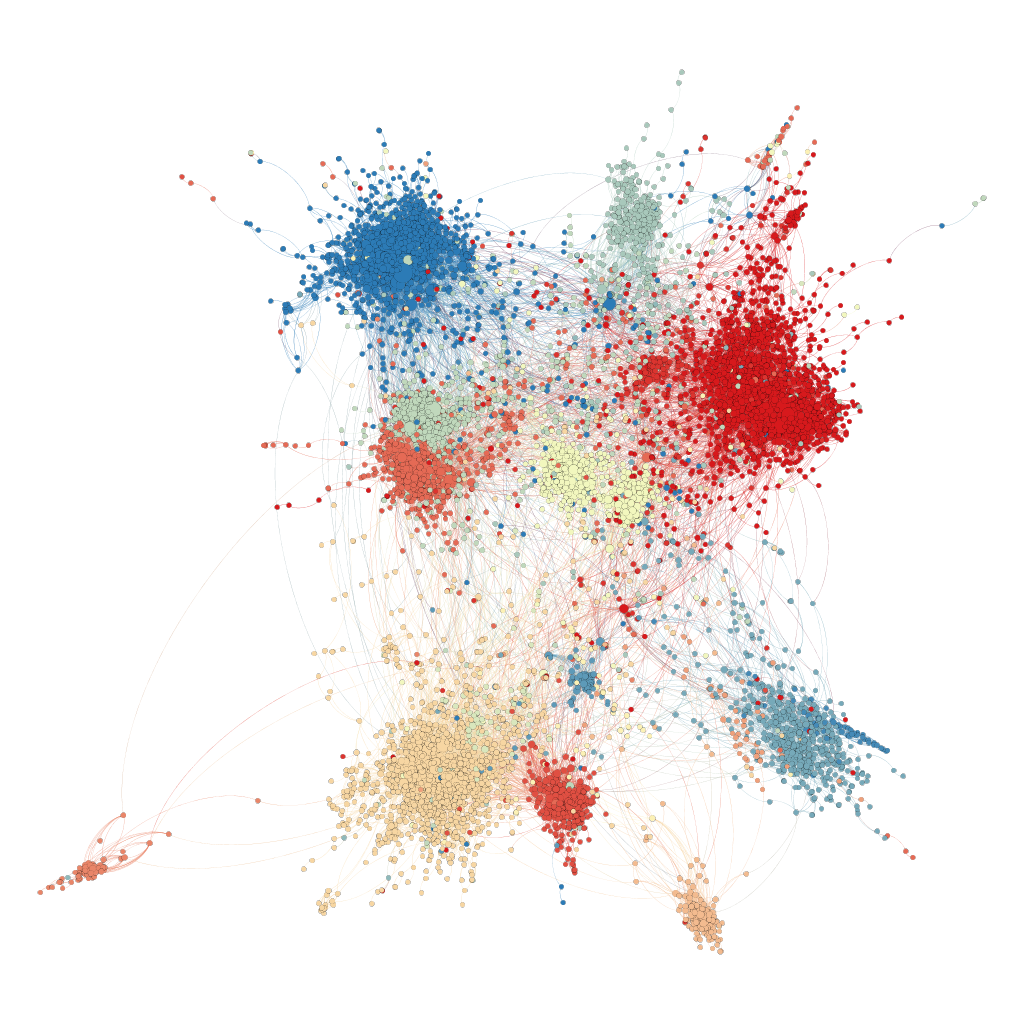
\includegraphics[width=1.097\textwidth]{img/resultados/grado-targets.png}
    \caption{Topología de la red. El color indica el país de cada usuario.}
\end{figure}

\begin{figure}[t]
    \centering
    \resizebox{0.78\columnwidth}{!}{%
    \begin{tabular}{| l | r |} 
        \hline
        \textbf{Medida} & \textbf{Valor} \\
        \Xhline{2\arrayrulewidth}
        Número de nodos \textbf{N} & 7,624 \\
        \hline
        Número de enlaces \textbf{L}	& 27,806 \\
        \hline
        Número máximo de enlaces \textbf{$L_{max}$} & 58117752 \\
        \hline
        Densidad del grafo \textbf{$L/L_{max}$} & 0.001 \\
        \Xhline{2\arrayrulewidth}
        Grado medio \textbf{<k>} & 7.294 \\
        \hline
        Diámetro \textbf{$d_{max}$} & 15 \\
        \hline
        Distancia media \textbf{d} & 5.232237269 \\
        \hline
        Coeficiente medio de clustering \textbf{<C>} & 0.285 \\
        \Xhline{2\arrayrulewidth}
        Número de componentes conexas & 1 \\
        \hline
        Número de nodos componente gigante (y \%) & 7,624 (100) \\
        \hline
        Número de aristas componente gigante (y \%) & 27,806 (100) \\
        \hline
    \end{tabular}
    }
    \caption{Medidas globales de la red.}
\end{figure} \newpage

    % ==============================================================================

    \setlength{\parskip}{1em}
    \newpage
    % \nocite{*}
    % \bibliography{bibliografia}
  	% \bibliographystyle{plain}
\end{document}